\section{Besturing op Afstand}

Een test van een motor kan mogelijk lang duren het zou hierbij makkelijk kunnen zijn om vanaf afstand de motor te testen. Ook is het gemakkelijk bij het modificeren van de testkast om dit vanaf afstand te doen. Dit is mogelijk via \gls{TwinCAT} routes. Via internet is het mogelijk om de testkast te besturen zolang er \gls{TwinCAT} geïnstalleerd is op de computer. Dit hoofdstuk is een how-to voor het verbinden van de testkast met een externe computer.

\subsection{\gls{TwinCAT} Installatie}

Om met de testkast te verbinden is het verreist om TwinCAT geïnstalleerd te hebben op de computer. Alleen \gls{TwinCAT} XAR is voldoende om via \gls{ADS} te verbinden met de testkast dit kan met de tutorial in bijlage \ref{sec:TwinCATInstallatie}.

\subsection{\gls{TwinCAT} Routes}

Wanneer \gls{TwinCAT} XAR geïnstalleerd is, is het mogelijk om te gaan verbinden met de testkast dit kan door eerst op het \gls{TwinCAT} icoontje te drukken zoals in figuur \ref{fig:TwinCATIcon}.


\begin{figure}[H]
	\centering
	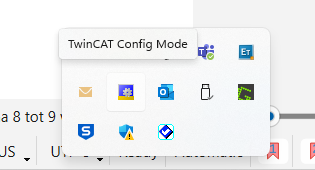
\includegraphics[width=0.7\linewidth]{TwinCATRoutes}
	\caption{\gls{TwinCAT} icon}
	\label{fig:TwinCATIcon}
\end{figure}

\newpage

Ga hierna naar de routes tool om een route te maken naar de testkast waar het test programma over kan praten met de testkast (figuur \ref{fig:Routes}). Er kan een route worden toegevoegd door op \textit{Add...} te drukken waarna er een scherm zal verschijnen waar men kan zoeken naar andere computers. Wanneer het IP-address van de testkast ingevuld wordt zal deze verschijnen. Voeg de testkast dan toe door er op te klikken en door op \textit{Add Route} te drukken. Zorg er uiteraard wel voor dat de route is verbonden anders kan de spindeltester niet connecten met de testkast. Een uitgebreidere how-to is ook wel te vinden op de site van beckhoff (bijlage \ref{sec:TwinCATRoutes})

\vspace{0.5cm}

Om het IP-address van de testkast te achterhalen kan men het volgende command typen in command prompt: \textit{ipconfig /all}. Let op dat het IP-address van de testkast nog wel eens kan veranderen. Het IP-address zal staan op het IPv4 Address ook wel te zien in figuur \ref{fig:IPAddress}.

 \begin{figure}[H]
 	\centering
 	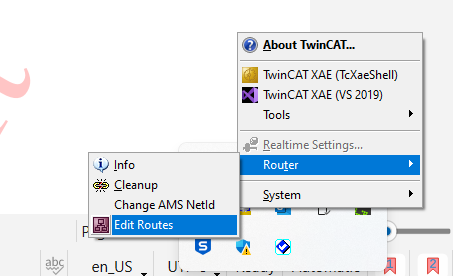
\includegraphics[width=0.7\linewidth]{Routes}
 	\caption{\gls{TwinCAT} Routes}
 	\label{fig:Routes}
 \end{figure}
 
 \begin{figure}[H]
 	\centering
 	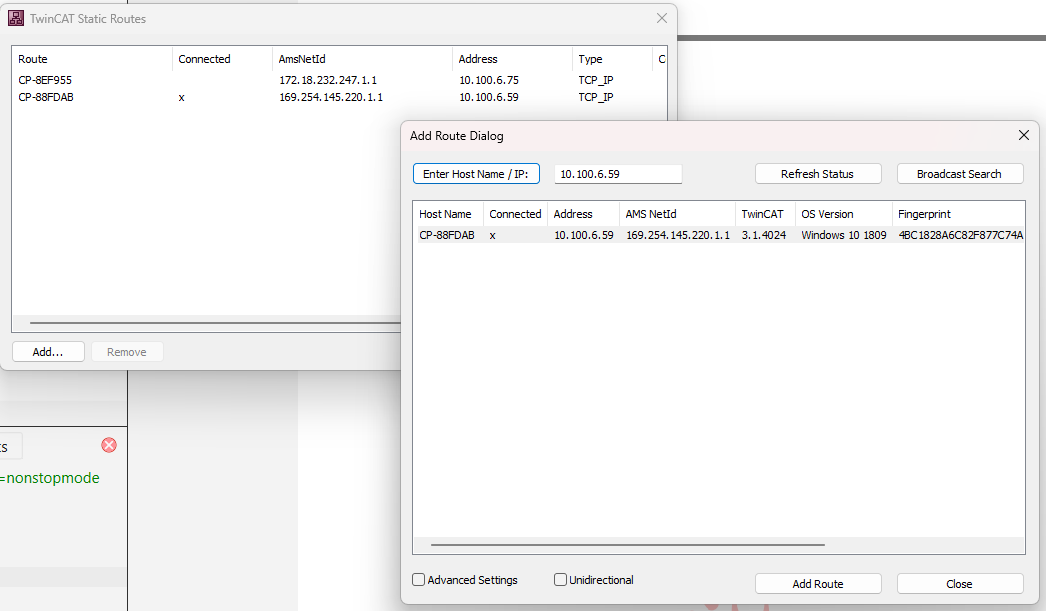
\includegraphics[width=\linewidth]{Routes2}
 	\caption{\gls{TwinCAT} Routes}
 	\label{fig:Routes2}
 \end{figure}
 
  \begin{figure}[H]
 	\centering
 	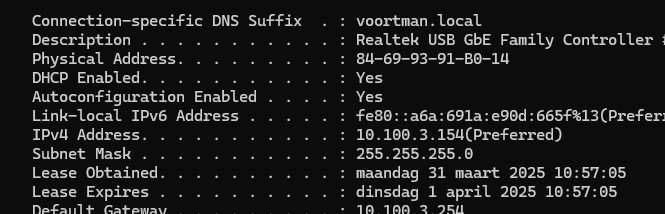
\includegraphics[width=\linewidth]{IPAddress}
 	\caption{IP-Address}
 	\label{fig:IPAddress}
 \end{figure}
 
 Run tot slot de installer van de spindel tester \textit{SpindleTesterSetup.exe} deze zou automatisch het spindel tester programma moeten installeren waarna de spindel direct kan worden bestuurt vanaf een andere computer.
 
 
	